%\documentclass[ckj,dvipdfmx]{beamer}
\documentclass[ckj,dvipdfmx]{beamer}
\usepackage{etex}
%\usetheme{Warsaw}
\usetheme{Malmoe}
%\usetheme{AnnArbor}
%\usetheme{Hannover}
%\usetheme{Bergen}
%\usetheme{Berlin}
%\usetheme{Singapore}
%\usetheme{Montpellier}
%\usetheme{Pittsburgh}
\usepackage{graphicx}
\usepackage{latexsym,amssymb}
%\usepackage{epsbox}
%\usepackage{multirow}
%\usepackage{fancybox}
\usepackage{tikz}
\usetikzlibrary{calc}
\usepackage{fancyvrb}
%\usepackage{listings}
\usepackage{tabularx}
%\usepackage{pstricks,pst-node,pst-tree}
%\usepackage{multimedia}
%\usepackage{pstricks,pst-node,pst-tree}
%\usepackage{pst-all}
%\include{prooftree}
%\lstloadlanguages{pascal}
\usepackage{mathrsfs}
\renewcommand{\kanjifamilydefault}{\gtdefault}
\renewcommand{\familydefault}{\sfdefault}

\newcommand{\greentext}[1]{{\color[rgb]{0,0.5,0}{#1}}}
\newcommand{\redtext}[1]{{\color[rgb]{0.8,0,0}{#1}}}
\newcommand{\bluetext}[1]{{\color[rgb]{0,0,0.8}{#1}}}

\newcommand{\tuple}[1]{\langle{#1}\rangle}

\newcommand{\First}{\mathsf{First}_1}
\newcommand{\Follow}{\mathsf{Follow}_1}

%%pdt simulation

\newcommand{\pdtline}[6]{%
    \uncover<#6->{
    \node at (${#5}*(0,-.3)+(0,.3)$) {$\vdash$};%
    \node at (${#5}*(0,-.3)+(1.5,.3)$) {\parbox{12em}{(#1,}};%
    \node at (${#5}*(0,-.3)+(4.5,.3)$) {\parbox{10em}{#2,}};%
    \node at (${#5}*(0,-.3)+(5.7,.3)$) {\parbox{10em}{#3)}};%
    \node at (${#5}*(0,-.3)+(8,.3)$) {\parbox{20em}{#4}};%
    }
}

\newcommand{\initpdtline}[6]{%
    \uncover<#6->{
    \node at (${#5}*(0,-.3)+(1.5,.3)$) {\parbox{12em}{(#1,}};%
    \node at (${#5}*(0,-.3)+(4.5,.3)$) {\parbox{10em}{#2,}};%
    \node at (${#5}*(0,-.3)+(5.7,.3)$) {\parbox{10em}{#3)}};%
    \node at (${#5}*(0,-.3)+(8,.3)$) {\parbox{20em}{#4}};%
    }
}

\newtheorem{Def}{定義}
\newtheorem{Lem}{補題}
\newtheorem{Thm}{定理}
\newtheorem{Prop}{命題}

\definecolor{lightlightgrey}{rgb}{0.95,0.95,0.95}
\definecolor{darkgreen}{rgb}{0,0.64,0}

\newcommand{\vdom}{\underline{\gg}}
\newcommand{\svdom}{\gg}

\newcommand{\ttpl}{\texttt{+}}
\newcommand{\ttsb}{\texttt{-}}
\newcommand{\ttmu}{\texttt{*}}
\newcommand{\ttdv}{\texttt{/}}
%\include{cmacros}

%\newcommand{\greentext}[1]{{\color[rgb]{0,0.5,0}{#1}}}
%\newcommand{\redtext}[1]{{\color[rgb]{0.8,0,0}{#1}}}

\newcommand{\lecturedate}{2026/11/24}

%\cornersize{0.25}
\graphicspath{{figs261124/}}

\setbeamertemplate{frametitle}[default][center]
\setbeamertemplate{footline}{\hfill
コンパイラ\quad\lecturedate
\hfill\insertframenumber/\inserttotalframenumber\hspace*{1zw}}
\newcounter{coffee}
\setbeamercovered{transparent=10}
\title{コンパイラ(14)}
\date{\lecturedate}
\begin{document}
\frame{\titlepage}

\begin{frame}
 \begin{center}
  {\Huge 目的コード生成}
 \end{center}
\end{frame}

\section{目的コード生成}

\begin{frame}
 \frametitle{目的コード生成}

 \begin{list}{}{}
  \item [フロントエンド] 構文木$\rightarrow$3番地コード
  \item [バックエンド] 3番地コード$\rightarrow$目的コード\\
	命令コード(ほぼ3番地コード)\\
	レジスタ割当(7.1,7.2)
	\begin{list}{}{}
	 \item [7.1] 木構造に対するレジスタ利用解析
	 \item [7.2] グラフ彩色によるレジスタ割当
	\end{list}
 \end{list}

\end{frame}

\subsection{レジスタ利用解析}

\begin{frame}[fragile]
  \frametitle{レジスタ利用解析}
  \greentext{四則演算式の抽象構文木から計算に必要なレジスタ数を算出}\\

  \vspace*{3mm}

  \greentext{木構造の演算式では複雑なフロー解析は不要}

  \vspace*{3mm}

  \begin{tabular}{llll}
  Load命令 & $\mathsf{Load}\ r,e$ & ($e$ $\rightarrow$ $r$)\\[5pt]
  演算命令 & $\theta\ r,e$ & ($r\theta e\rightarrow r$) & $\theta\in\{\ttpl,\ttsb,\ttmu,\ttdv\}$
  \end{tabular}

  \vspace*{5mm}

  \only<1>{
  \begin{tabular}{cccc}
  \begin{minipage}{.22\textwidth}
    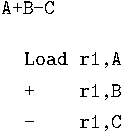
\includegraphics{expression1-crop.pdf}
  \end{minipage}
  &
  \begin{minipage}{.18\textwidth}
    \scalebox{0.75}{
    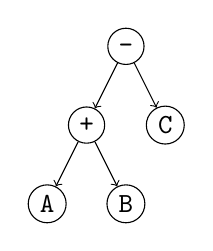
\begin{tikzpicture}
      \node[draw,circle,inner sep=2pt] (N0) at (0,0) {\texttt{A}};
      \node[draw,circle,inner sep=2pt] (N1) at (1,0) {\texttt{B}};
      \node[draw,circle,inner sep=2pt] (N2) at (0.5,1) {\texttt{+}};
      \node[draw,circle,inner sep=2pt] (N3) at (1.5,1) {\texttt{C}};
      \node[draw,circle,inner sep=2pt] (N4) at (1,2) {\texttt{-}};
      \path[->] (N2) edge (N0) (N2) edge (N1) (N4) edge (N2) (N4) edge (N3);
    \end{tikzpicture}}
  \end{minipage}
  &
  \begin{minipage}{.22\textwidth}
      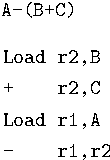
\includegraphics{expression2-crop.pdf}
    \end{minipage}
  &
  \begin{minipage}{.18\textwidth}
  \scalebox{0.75}{
  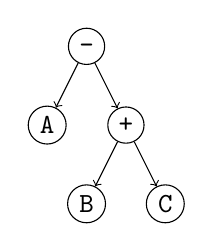
\begin{tikzpicture}
    \node[draw,circle,inner sep=2pt] (N0) at (0.5,1) {\texttt{A}};
    \node[draw,circle,inner sep=2pt] (N1) at (1,0) {\texttt{B}};
    \node[draw,circle,inner sep=2pt] (N2) at (1,2) {\texttt{-}};
    \node[draw,circle,inner sep=2pt] (N3) at (2,0) {\texttt{C}};
    \node[draw,circle,inner sep=2pt] (N4) at (1.5,1) {\texttt{+}};
    \path[->] (N2) edge (N0) (N2) edge (N4) (N4) edge (N1) (N4) edge (N3);
  \end{tikzpicture}}
  \end{minipage}\\[35pt]
  \multicolumn{2}{c}{$RN(T_1)=1$} &
  \multicolumn{2}{c}{$RN(T_2)=2$}
\end{tabular}
  }
  \only<2>{
\begin{tabular}{cccc}
  \begin{minipage}{.22\textwidth}
    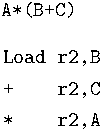
\includegraphics{expression3-crop.pdf}
  \end{minipage}
  &
  \begin{minipage}{.18\textwidth}
    \scalebox{0.75}{
    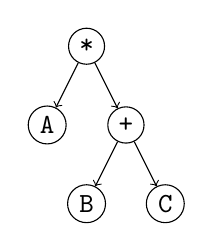
\begin{tikzpicture}
      \node[draw,circle,inner sep=2pt] (N0) at (0.5,1) {\texttt{A}};
      \node[draw,circle,inner sep=2pt] (N1) at (1,0) {\texttt{B}};
      \node[draw,circle,inner sep=2pt] (N2) at (1,2) {\texttt{*}};
      \node[draw,circle,inner sep=2pt] (N3) at (2,0) {\texttt{C}};
      \node[draw,circle,inner sep=2pt] (N4) at (1.5,1) {\texttt{+}};
      \path[->] (N2) edge (N0) (N2) edge (N4) (N4) edge (N1) (N4) edge (N3);
    \end{tikzpicture}}
    \end{minipage}
  &
  \begin{minipage}{.22\textwidth}
      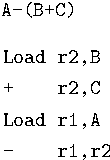
\includegraphics{expression2-crop.pdf}
    \end{minipage}
  &
  \begin{minipage}{.18\textwidth}
  \scalebox{0.75}{
  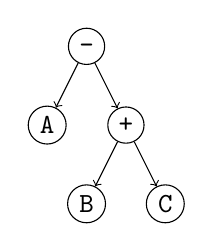
\begin{tikzpicture}
    \node[draw,circle,inner sep=2pt] (N0) at (0.5,1) {\texttt{A}};
    \node[draw,circle,inner sep=2pt] (N1) at (1,0) {\texttt{B}};
    \node[draw,circle,inner sep=2pt] (N2) at (1,2) {\texttt{-}};
    \node[draw,circle,inner sep=2pt] (N3) at (2,0) {\texttt{C}};
    \node[draw,circle,inner sep=2pt] (N4) at (1.5,1) {\texttt{+}};
    \path[->] (N2) edge (N0) (N2) edge (N4) (N4) edge (N1) (N4) edge (N3);
  \end{tikzpicture}}
  \end{minipage}\\[35pt]
  \multicolumn{2}{c}{$RN(T_1)=1$} &
  \multicolumn{2}{c}{$RN(T_2)=2$}
\end{tabular}
  }

  \only<2>{\redtext{乗算は可換であるため}}
\end{frame}

\begin{frame}
\frametitle{レジスタ数の見積:$RN$}
{\scriptsize
  \begin{list}{}{}
  \item $T$が葉のとき：$RN(T)=0$
  \item $T$が葉以外のとき：
  \greentext{$T_1$:$T$の左部分木，$T_2$:$T$の右部分木とする}
  \begin{list}{}{}
    \item $RN(T_1)=RN(T_2)=0$のとき，$RN(T)=1$
    \item $RN(T_1)=0$,$RN(T_2)>0$のとき，
    \begin{list}{}{}
      \item $\mathsf{root}(T)$が可換演算ならば$RN(T)=RN(T_2)$
      \item $\mathsf{root}(T)$が可換でないとき$RN(T)=\max(2,RN(T_2))$
    \end{list}
  \item $RN(T_1)>0$のとき
  \begin{list}{}{}
    \item $RN(T_1)=RN(T_2)$のとき, $RN(T)=RN(T_1)+1$
    \item $RN(T_1)\not= RN(T_2)$のとき，$RN(T)=\max(RN(T_1),RN(T_2))$
  \end{list}
\end{list}
\end{list}
}
\end{frame}

\begin{frame}
  \frametitle{式のコード生成:$\mathsf{Code}(T,(r_1,\cdots,r_k))$}
  {\scriptsize
  \begin{list}{}{}
    \item $T$が葉のとき：何もしない
    \item $T$が葉でないとき：
    \begin{list}{}{}
      \item $RN(T_1)=RN(T_2)=0$のとき：\\
      \quad $\mathsf{output}$(\texttt{Load},$r_1$,$T_1$);$\mathsf{output}$($\theta$,$r_1$,$T_2$);
      \item $RN(T_1)=0,RN(T_2)>0$のとき：
      \begin{list}{}{}
        \item $\mathsf{root}(T)$が可換のとき:\\
        \quad $\mathsf{Code}$($T_2$,($r_1$,$\cdots$,$r_k$));
        $\mathsf{output}$($\theta$,$r_1$,$T_1$);
        \item $\mathsf{root}(T)$が可換でないとき:\\
        \quad $\mathsf{Code}$($T_2$,($r_2$,$\cdots$,$r_k$));
        $\mathsf{output}$(\texttt{Load},$r_1$,$T_1$);
        $\mathsf{output}$($\theta$,$r_1$,$r_2$);
      \end{list}
      \item $RN(T_1)>0,RN(T_2)=0$のとき：\\
      \quad $\mathsf{Code}$($T_1$,($r_1$,$\cdots$,$r_k$));
      $\mathsf{output}$($\theta$,$r_1$,$T_2$);
      \item $RN(T_1)>0,RN(T_2)>0$のとき：
      \begin{list}{}{}
        \item $RN(T_1)\geq RN(T_2)$のとき：\\
        \quad $\mathsf{Code}$($T_1$,($r_1$,$\cdots$,$r_k$));
        $\mathsf{Code}$($T_2$,($r_2$,$\cdots$,$r_k$));
        $\mathsf{output}$($\theta$,$r_1$,$r_2$);
        \item $RN(T_1)<RN(T_2)$のとき：\\
        \quad $\mathsf{Code}$($T_2$,($r_2$,$\cdots$,$r_k$,$r_1$));
        $\mathsf{Code}$($T_1$,($r_1$,$r_3$,$\cdots$,$r_k$));
        $\mathsf{output}$($\theta$,$r_1$,$r_2$);
      \end{list}
    \end{list}
  \end{list}
  }
\end{frame}

\begin{frame}
  \frametitle{コード生成例}
  \begin{tikzpicture}
  \node[draw,circle,inner sep=2pt] (T1) at (0,0) {\ttdv};
  \node[draw,circle,inner sep=2pt] (T2) at (-1,-1) {\ttpl};
  \node[draw,circle,inner sep=2pt] (T3) at (1,-1) {\ttsb};
  \node[draw,circle,inner sep=2pt] (T4) at (-1.5,-2) {\ttmu};
  \node[draw,circle,inner sep=2pt] (T5) at (-0.5,-2) {\texttt{C}};
  \node[draw,circle,inner sep=2pt] (T6) at (0.5,-2) {\texttt{D}};
  \node[draw,circle,inner sep=2pt] (T7) at (1.5,-2) {\texttt{E}};
  \node[draw,circle,inner sep=2pt] (T8) at (-2,-3) {\texttt{A}};
  \node[draw,circle,inner sep=2pt] (T9) at (-1,-3) {\texttt{B}};
  \path[->] (T1) edge (T2) (T1) edge (T3);
  \path[->] (T2) edge (T4) (T2) edge (T5);
  \path[->] (T3) edge (T6) (T3) edge (T7);
  \path[->] (T4) edge (T8) (T4) edge (T9);

  \node at ($(T1)+(0,1)$) {\texttt{(A*B+C)/(D-E)}};
  
  \node at ($(T4)+(0.4,0.1)$) {\greentext{$T_1$}};
  \node at ($(T2)+(0.4,0.1)$) {\greentext{$T_2$}};
  \node at ($(T3)+(0.4,0.1)$) {\greentext{$T_3$}};
  \node at ($(T1)+(0.4,0.1)$) {\greentext{$T_4$}};
  \only<2->{\node at ($(T8)+(-0.35,0.1)$) {\redtext{\scriptsize 0}};
  \node at ($(T9)+(0.35,0.1)$) {\redtext{\scriptsize 0}};
  \node at ($(T5)+(0.35,0.1)$) {\redtext{\scriptsize 0}};
  \node at ($(T6)+(-0.35,0.1)$) {\redtext{\scriptsize 0}};
  \node at ($(T7)+(0.35,0.1)$) {\redtext{\scriptsize 0}};
  }
  \only<3->{
    \node at ($(T4)+(-0.35,0.1)$) {\redtext{\scriptsize 1}};
    \node at ($(T3)+(-0.35,0.1)$) {\redtext{\scriptsize 1}};
  }
  \only<4->{
    \node at ($(T2)+(-0.35,0.1)$) {\redtext{\scriptsize 1}};
  }
  \only<5->{
    \node at ($(T1)+(-0.35,0.1)$) {\redtext{\scriptsize 2}};
  }
  \only<6>{
    \node[anchor=north west] (C1) at ($(T1)+(3,1)$) {\begin{tabular}{l}
      $\mathsf{Code}(T_4,(r_1,r_2))$\end{tabular}};
  }
  \only<7>{
    \node[anchor=north west] (C1) at ($(T1)+(3,1)$) {\begin{tabular}{l}
      $\mathsf{Code}(T_2,(r_1))$\\
      $\mathsf{Code}(T_3,(r_2))$\\
      $\mathsf{output}(\ttdv,r_1,r_2)$
    \end{tabular}};
  }
  \only<8>{
    \node[anchor=north west] (C1) at ($(T1)+(3,1)$) {\begin{tabular}{l}
      $\mathsf{Code}(T_1,(r_1))$\\
      $\mathsf{output}(\ttpl,r_1,\texttt{C})$\\
      $\mathsf{Code}(T_3,(r_2))$\\
      $\mathsf{output}(\ttdv,r_1,r_2)$
    \end{tabular}};
  }
  \only<9>{
    \node[anchor=north west] (C1) at ($(T1)+(3,1)$) {\begin{tabular}{l}
      $\mathsf{output}(\texttt{Load},r_1,\texttt{A})$\\
      $\mathsf{output}(\ttmu,r_1,\texttt{B})$\\
      $\mathsf{output}(\ttpl,r_1,\texttt{C})$\\
      $\mathsf{Code}(T_3,(r_2))$\\
      $\mathsf{output}(\ttdv,r_1,r_2)$
    \end{tabular}};
  }
  \only<10>{
    \node[anchor=north west] (C1) at ($(T1)+(3,1)$) {\begin{tabular}{l}
      $\mathsf{output}(\texttt{Load},r_1,\texttt{A})$\\
      $\mathsf{output}(\ttmu,r_1,\texttt{B})$\\
      $\mathsf{output}(\ttpl,r_1,\texttt{C})$\\
      $\mathsf{output}(\texttt{Load},r_2,\texttt{D})$\\
      $\mathsf{output}(\ttsb,r_2,\texttt{E})$\\
      $\mathsf{output}(\ttdv,r_1,r_2)$
    \end{tabular}};
  }
  \end{tikzpicture}
\end{frame}

\begin{frame}
  \frametitle{コード生成例}
  \begin{tikzpicture}
    \node[draw,circle,inner sep=2pt] (S1) at (0,0) {\ttpl};
    \node[draw,circle,inner sep=2pt] (S2) at (-1,-1) {\ttdv};
    \node[draw,circle,inner sep=2pt] (S3) at (1,-1) {\ttsb};
    \node[draw,circle,inner sep=2pt] (S4) at (-1.5,-2) {\texttt{A}};
    \node[draw,circle,inner sep=2pt] (S5) at (-0.5,-2) {\ttmu};
    \node[draw,circle,inner sep=2pt] (S6) at (0.5,-2) {\texttt{D}};
    \node[draw,circle,inner sep=2pt] (S7) at (1.5,-2) {\ttdv};
    \node[draw,circle,inner sep=2pt] (S8) at (-1,-3) {\texttt{B}};
    \node[draw,circle,inner sep=2pt] (S9) at (0,-3) {\texttt{C}};
    \node[draw,circle,inner sep=2pt] (S10) at (1,-3) {\texttt{E}};
    \node[draw,circle,inner sep=2pt] (S11) at (2,-3) {\texttt{F}};
    \node at ($(S1)+(0,1)$) {\texttt{A/(B*C)+(D-E/F)}};
    \path[->] (S1) edge (S2) (S1) edge (S3);
    \path[->] (S2) edge (S4) (S2) edge (S5);
    \path[->] (S3) edge (S6) (S3) edge (S7);
    \path[->] (S5) edge (S8) (S5) edge (S9);
    \path[->] (S7) edge (S10) (S7) edge (S11);

    \only<3->{
    \node at ($(S5)+(0.25,0.25)$) {\greentext{$T_1$}};
    \node at ($(S7)+(0.25,0.25)$) {\greentext{$T_2$}};
    \node at ($(S2)+(0.25,0.25)$) {\greentext{$T_3$}};
    \node at ($(S3)+(0.25,0.25)$) {\greentext{$T_4$}};
    \node at ($(S1)+(0.25,0.25)$) {\greentext{$T_5$}};
    }
    \only<2->{
    \node at ($(S1)+(-0.35,0.1)$) {\redtext{3}}; 
    \node at ($(S2)+(-0.35,0.1)$) {\redtext{2}};
    \node at ($(S3)+(-0.35,0.1)$) {\redtext{2}};
    \node at ($(S4)+(-0.35,0.1)$) {\redtext{0}}; 
    \node at ($(S5)+(-0.35,0.1)$) {\redtext{1}};
    \node at ($(S6)+(-0.35,0.1)$) {\redtext{0}};
    \node at ($(S7)+(-0.35,0.1)$) {\redtext{1}};
    \node at ($(S8)+(-0.35,0.1)$) {\redtext{0}}; 
    \node at ($(S9)+(-0.35,0.1)$) {\redtext{0}};
    \node at ($(S10)+(-0.35,0.1)$) {\redtext{0}};
    \node at ($(S11)+(-0.35,0.1)$) {\redtext{0}};
    }
    \only<4>{
      \node[anchor=north west] at ($(S1)+(3,1)$) {
        \begin{tabular}{l}$\mathsf{Code}(T_5,(r_1,r_2,r_3))$\end{tabular}
      };
    }
    \only<5>{
      \node[anchor=north west] at ($(S1)+(3,1)$) {
        \begin{tabular}{l}$\mathsf{Code}(T_3,(r_1,r_2,r_3))$\\
          $\mathsf{Code}(T_4,(r_2,r_3))$\\
          $\mathsf{output}(\ttpl,r_1,r_2)$
        \end{tabular}
      };
    }
    \only<6>{
      \node[anchor=north west] at ($(S1)+(3,1)$) {
        \begin{tabular}{l}$\mathsf{Code}(T_1,(r_2))$\\
          $\mathsf{output}(\texttt{Load},r_1,\texttt{A})$\\
          $\mathsf{output}(\ttdv,r_1,r_2)$\\
          $\mathsf{Code}(T_4,(r_2,r_3))$\\
          $\mathsf{output}(\ttpl,r_1,r_2)$
        \end{tabular}
      };
    }
    \only<7>{
      \node[anchor=north west] at ($(S1)+(3,1)$) {
        \begin{tabular}{l}
          $\mathsf{output}(\texttt{Load},r_2,\texttt{B})$\\
          $\mathsf{output}(\ttmu,r_2,\texttt{C})$\\
          $\mathsf{output}(\texttt{Load},r_1,\texttt{A})$\\
          $\mathsf{output}(\ttdv,r_1,r_2)$\\
          $\mathsf{Code}(T_4,(r_2,r_3))$\\
          $\mathsf{output}(\ttpl,r_1,r_2)$
        \end{tabular}
      };
    }
    \only<8>{
      \node[anchor=north west] at ($(S1)+(3,1)$) {
        \begin{tabular}{l}
          $\mathsf{output}(\texttt{Load},r_2,\texttt{B})$\\
          $\mathsf{output}(\ttmu,r_2,\texttt{C})$\\
          $\mathsf{output}(\texttt{Load},r_1,\texttt{A})$\\
          $\mathsf{output}(\ttdv,r_1,r_2)$\\
          $\mathsf{Code}(T_2,(r_3))$\\
          $\mathsf{output}(\texttt{Load},r_2,\texttt{D})$\\
          $\mathsf{output}(\ttsb,r_2,r_3)$\\
          $\mathsf{output}(\ttpl,r_1,r_2)$
        \end{tabular}
      };
    }
    \only<9>{
      \node[anchor=north west] at ($(S1)+(3,1)$) {
        \begin{tabular}{l}
          $\mathsf{output}(\texttt{Load},r_2,\texttt{B})$\\
          $\mathsf{output}(\ttmu,r_2,\texttt{C})$\\
          $\mathsf{output}(\texttt{Load},r_1,\texttt{A})$\\
          $\mathsf{output}(\ttdv,r_1,r_2)$\\
          $\mathsf{output}(\texttt{Load},r_3,\texttt{E})$\\
          $\mathsf{output}(\ttdv,r_3,\texttt{F})$\\
          $\mathsf{output}(\texttt{Load},r_2,\texttt{D})$\\
          $\mathsf{output}(\ttsb,r_2,r_3)$\\
          $\mathsf{output}(\ttpl,r_1,r_2)$
        \end{tabular}
      };
    }
  \end{tikzpicture}
\end{frame}

\subsection{レジスタ割当}

% \begin{frame}
%   \frametitle{レジスタ利用解析}
%   \greentext{四則演算式の抽象構文木から計算に必要なレジスタ数を算出}\\
%   Load命令 $\mathsf{Load}\ r,e$ ($e$ $\rightarrow$ $r$)\\
%   演算命令 $\theta\ r,e$ ($r\theta e\rightarrow r$)
% \end{frame}

\begin{frame}
  \frametitle{変数の生存解析}
  各命令$I_i$を基本ブロックとして生存解析
  $In[I_i]=Use[I_i]\cup(Out[I_i]-Def[I_i])$\\
  $Out[I_i]=In[I_{i+1}]$ ($1\leq i\leq 5$), $Out[I_6]=In[I_1]$

  \vspace*{10pt}

  \begin{tabular}{cc}
    \multicolumn{1}{m{.42\textwidth}}{
  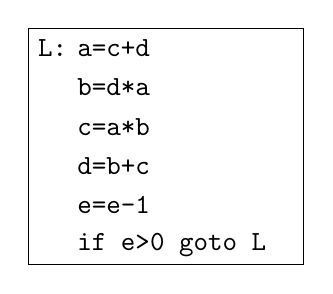
\begin{tikzpicture}
  \node[anchor=west] at (-0.5,2.5) {\texttt{L:}};
 	\node[anchor=west] at (0,2.5) {\texttt{a=c+d}};
 	\node[anchor=west] at (0,2) {\texttt{b=d*a}};
 	\node[anchor=west] at (0,1.5) {\texttt{c=a*b}};
 	\node[anchor=west] at (0,1) {\texttt{d=b+c}};
 	\node[anchor=west] at (0,0.5) {\texttt{e=e-1}};
 	\node[anchor=west] at (0,0) {\texttt{if e>0 goto L}};
 	\draw[anchor=west,draw] (-.5,-.25) rectangle +(3.5,3);
 \end{tikzpicture}}
 &

  \multicolumn{1}{m{.48\textwidth}}{
    \begin{tabular}{|c|cc|}\hline
      & IN & OUT\\\hline
    $I_1$ & $\{c,d,e\}$ & $\{a,d,e\}$\\
    $I_2$ & $\{a,d,e\}$ & $\{a,b,e\}$\\
    $I_3$ & $\{a,b,e\}$ & $\{b,c,e\}$\\
    $I_4$ & $\{b,c,e\}$ & $\{c,d,e\}$\\
    $I_5$ & $\{c,d,e\}$ & $\{c,d,e\}$\\
    $I_6$ & $\{c,d,e\}$ & $\{c,d,e\}$\\\hline
    \end{tabular}
  }
\end{tabular}
\end{frame}

\begin{frame}
  \frametitle{生存解析の詳細}
  \[\begin{array}{l}
    In[I_1]=\{c,d\}\cup(Out[I_1]-\{a\})\\
    Out[I_1]=In[I_2]=\{a,d\}\cup(Out[I_2]-\{b\})\\
    Out[I_2]=In[I_3]=\{a,b\}\cup(Out[I_3]-\{c\})\\
    Out[I_3]=In[I_4]=\{b,c\}\cup(Out[I_4]-\{d\})\\
    Out[I_4]=In[I_5]=\{e\}\cup(Out[I_5]-\{e\})\\
    Out[I_5]=In[I_6]=\{e\}\cup Out[I_6]\\
    Out[I_6]=In[I_1]
  \end{array}
    \]
  の方程式の解を求める．
  {\tiny
  \[\begin{array}{c|ccccccccccc}
    & OUT & IN & OUT & IN & OUT & IN & OUT & IN & OUT & IN & OUT\\\hline
  I_1 & 00000 & 00110 & 10010 & 00110 & 10010 & 00110 & 10010 & 00110 & 10011 & 00111 & 10011\\
  I_2 & 00000 & 10010 & 11000 & 10010 & 11000 & 10010 & 11001 & 10011 & 11001 & 10011 & 11001\\
  I_3 & 00000 & 11000 & 01100 & 11000 & 01101 & 11001 & 01101 & 11001 & 01101 & 11001 & 01101\\
  I_4 & 00000 & 01100 & 00001 & 01101 & 00001 & 01101 & 00111 & 01101 & 00111 & 01101 & 00111\\
  I_5 & 00000 & 00001 & 00001 & 00001 & 00111 & 00111 & 00111 & 00111 & 00111 & 00111 & 00111\\
  I_6 & 00000 & 00001 & 00110 & 00111 & 00110 & 00111 & 00110 & 00111 & 00110 & 00111 & 00111\\\hline
  \end{array}
    \]
  }
\end{frame}

\begin{frame}
 \frametitle{グラフ彩色アルゴリズムを用いたレジスタ割当て}
 
 基本ブロック内でのレジスタ割当

 \begin{list}{}{}
  \item [レジスタ干渉グラフ] $(V,E)$\\
	$V\subseteq X$，生存期間が重なる変数$u,v\in V$，$(u,v)\in
	E$\\
	生存期間：\greentext{変数が定義された時点からその定
	義が最後に使用される時点までの期間}
 \end{list}
 
 \begin{tabular}{cc}
 \begin{minipage}{.65\textwidth}
 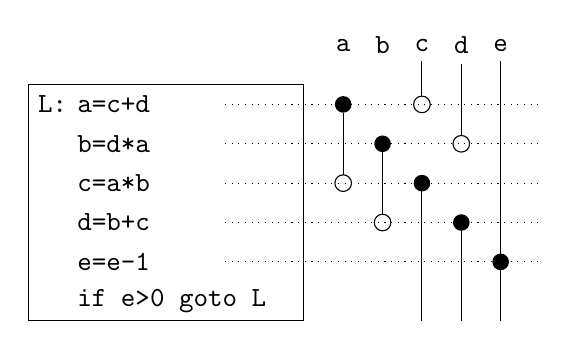
\begin{tikzpicture}
    \node at (3.5,3.25) {\texttt{a}};
    \node at (4,3.25) {\texttt{b}};
    \node (c0) at (4.5,3.25) {\texttt{c}};
    \node (d0) at (5,3.25) {\texttt{d}};
    \node (e0) at (5.5,3.25) {\texttt{e}};
  \node[anchor=west] at (-0.5,2.5) {\texttt{L:}};
 	\node[anchor=west] at (0,2.5) {\texttt{a=c+d}};
 	\node[anchor=west] at (0,2) {\texttt{b=d*a}};
 	\node[anchor=west] at (0,1.5) {\texttt{c=a*b}};
 	\node[anchor=west] at (0,1) {\texttt{d=b+c}};
 	\node[anchor=west] at (0,0.5) {\texttt{e=e-1}};
 	\node[anchor=west] at (0,0) {\texttt{if e>0 goto L}};
 	\path[-,style=dotted] (2,2.5) edge (6,2.5)
 	                      (2,2) edge (6,2)
 	                      (2,1.5) edge (6,1.5)
 	                      (2,1) edge (6,1)
 	                      (2,0.5) edge (6,0.5);
 	\draw[anchor=west,draw] (-.5,-.25) rectangle +(3.5,3);
 	\node[circle, fill, minimum size=6pt,inner sep=0pt,outer sep=0pt] (a0) at (3.5,2.5) {};
 	\node[draw,circle, minimum size=6pt,inner sep=0pt,outer sep=0pt] (a1) at (3.5,1.5) {};
 	\path[-] (a0) edge (a1);
  	\node[circle, fill, minimum size=6pt,inner sep=0pt,outer sep=0pt] (b0) at (4,2) {};
 	\node[draw,circle, minimum size=6pt,inner sep=0pt,outer sep=0pt] (b1) at (4,1) {};
 	\path[-] (b0) edge (b1);
  	\node[circle, fill, minimum size=6pt,inner sep=0pt,outer sep=0pt] (c1) at (4.5,1.5) {};
 	\node[draw,circle, minimum size=6pt,inner sep=0pt,outer sep=0pt] (c2) at (4.5,2.5) {};
    \path[-] (c0) edge (c2) (c1) edge (4.5,-0.25);
  	\node[circle, fill, minimum size=6pt,inner sep=0pt,outer sep=0pt] (d1) at (5,1) {};
 	\node[draw,circle, minimum size=6pt,inner sep=0pt,outer sep=0pt] (d2) at (5,2) {};
    \path[-] (d0) edge (d2) (d1) edge (5,-0.25);
  	\node[circle, fill, minimum size=6pt,inner sep=0pt,outer sep=0pt] (e1) at (5.5,0.5) {};
    \path[-] (e0) edge (e1) (e1) edge (5.5,-0.25);


 \end{tikzpicture}
 \end{minipage} &
  \begin{minipage}{.27\textwidth}
    \only<1>{
    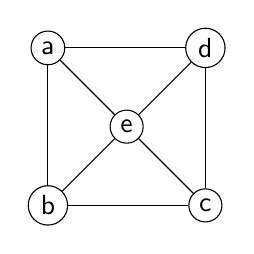
\begin{tikzpicture}
    \node[circle,inner sep=2pt,draw] (ar1) at (0,2) {a};
    \node[circle,inner sep=2pt,draw] (br1) at (0,0) {b};
    \node[circle,inner sep=2pt,draw] (cr1) at (2,0) {c};
    \node[circle,inner sep=2pt,draw] (dr1) at (2,2) {d};
    \node[circle,inner sep=2pt,draw] (er1) at (1,1) {e};
  	\path[-] (ar1) edge (br1) (ar1) edge (dr1) (ar1) edge (er1)
  	         (br1) edge (er1) (br1) edge (cr1) (dr1) edge (er1)
  	         (cr1) edge (er1) (cr1) edge (dr1);
  	\end{tikzpicture}
    }
    \only<2>{
    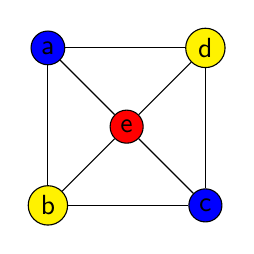
\begin{tikzpicture}
    \node[circle,inner sep=2pt,fill=blue,draw] (ar2) at (0,2) {a};
    \node[circle,inner sep=2pt,fill=yellow,draw] (br2) at (0,0) {b};
    \node[circle,inner sep=2pt,fill=blue,draw] (cr2) at (2,0) {c};
    \node[circle,inner sep=2pt,fill=yellow,draw] (dr2) at (2,2) {d};
    \node[circle,inner sep=2pt,fill=red,draw] (er2) at (1,1) {e};

  	\path[-] (ar2) edge (br2) (ar2) edge (dr2) (ar2) edge (er2)
  	         (br2) edge (er2) (br2) edge (cr2) (dr2) edge (er2)
  	         (cr2) edge (er2) (cr2) edge (dr2);
  	  \end{tikzpicture}
  	}
  \end{minipage}
  \end{tabular}
\end{frame}

\begin{frame}
 \frametitle{彩色問題とレジスタ割当}
 \begin{Def}
  無向グラフ$G=(V,E)$において，すべての辺$(u,v)\in E$に対して，
  $f(u)\not=f(v)$となる割当関数$f:V\rightarrow\{1,\cdots,k\}$
  が存在するとき，$G$は$k$-彩色可能である．
 \end{Def}
 先の例：3-彩色可能

 \vspace*{1zw}

 変数干渉グラフが$k$-彩色可能$\Leftrightarrow$ $k$個のレジス
 タに割当可能

 \vspace*{1zw}

 生存期間が重なる変数に同じレジスタを割り当てない

 \vspace*{1zw}

 グラフの$k$-彩色問題は一般にNP完全問題

 \vspace*{1zw}

 NP完全問題:\greentext{組合せをすべて試す必要がある問題}\\
 \greentext{グラフのノード数が増えると組合せが指数的に爆発的に増加}

 \vspace*{1zw}

 \redtext{レジスタを最適に割り当てて高速化することは現実的でない}
\end{frame}

\begin{frame}
 \frametitle{k-彩色アルゴリズム}
 \begin{Thm}
  $G=(V,E)$の任意の頂点の次数が$k-1$以下であれば，$k\ge
  1$となる$k$に対して$k$-彩色可能である．
 \end{Thm}

 証明は，$|V|$に関する帰納法．

 \greentext{アイデアは簡単．証明は彩色関数が実際に構成できる
 ことを示す．}
 
\end{frame}

\begin{frame}
 \frametitle{彩色アルゴリズム:準備}

 $G=(V,E)$の独立集合$I$：$(u,v)\in E$に対して，$u\in I$ならば
 $v\notin I$

 \vspace*{1zw}

 \only<1>{
 最大独立集合：要素数が最大の独立集合\\
 \quad\greentext{\small 一般に最大独立集合を求める問題はNP完
 全}\\
 \quad\greentext{\small 極大独立集合:$\mathsf{maxidp(G)}$：ひとつでも要
 素を加えると独立でなくなる}\\
 \begin{center}
  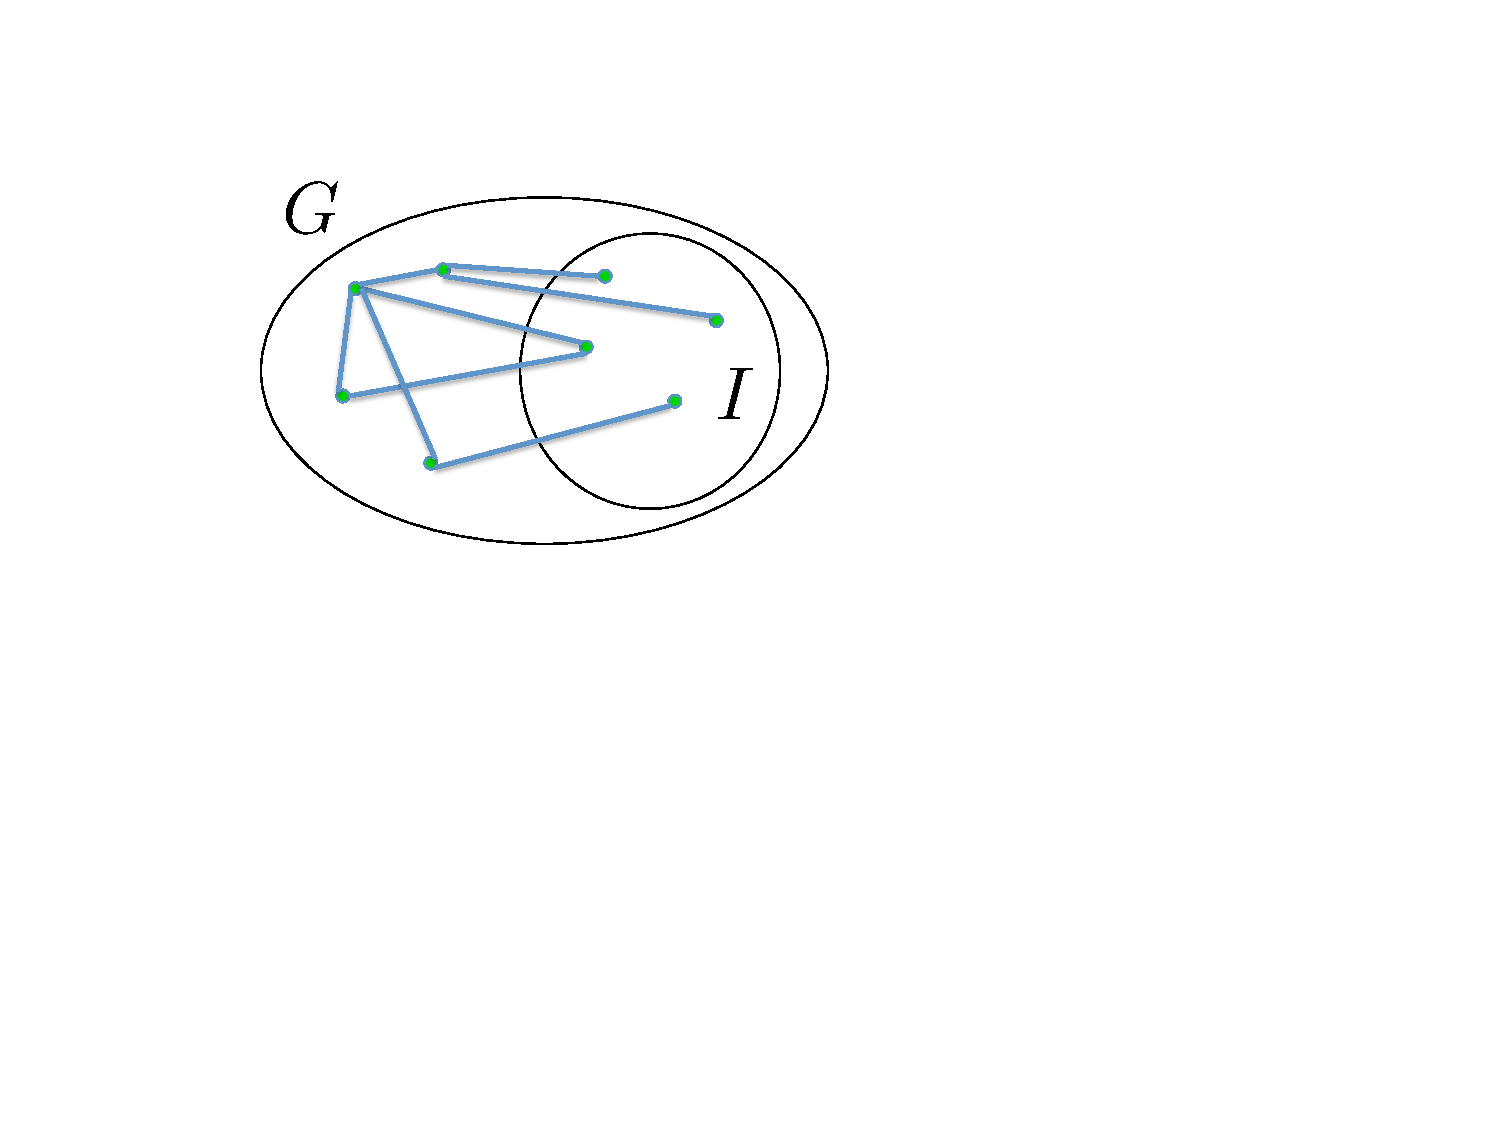
\includegraphics[scale=0.4]{idepmax01.pdf}
 \end{center}
 }
 
 \only<2>{
 最大独立集合：要素数が最大の独立集合\\
 \quad\greentext{\small 二部グラフの場合は多項式時間で求められる．}\\
 \quad\greentext{\small 極大独立集合:$\mathsf{maxidp(G)}$：ひとつでも要
 素を加えると独立でなくなる}\\
 \begin{center}
  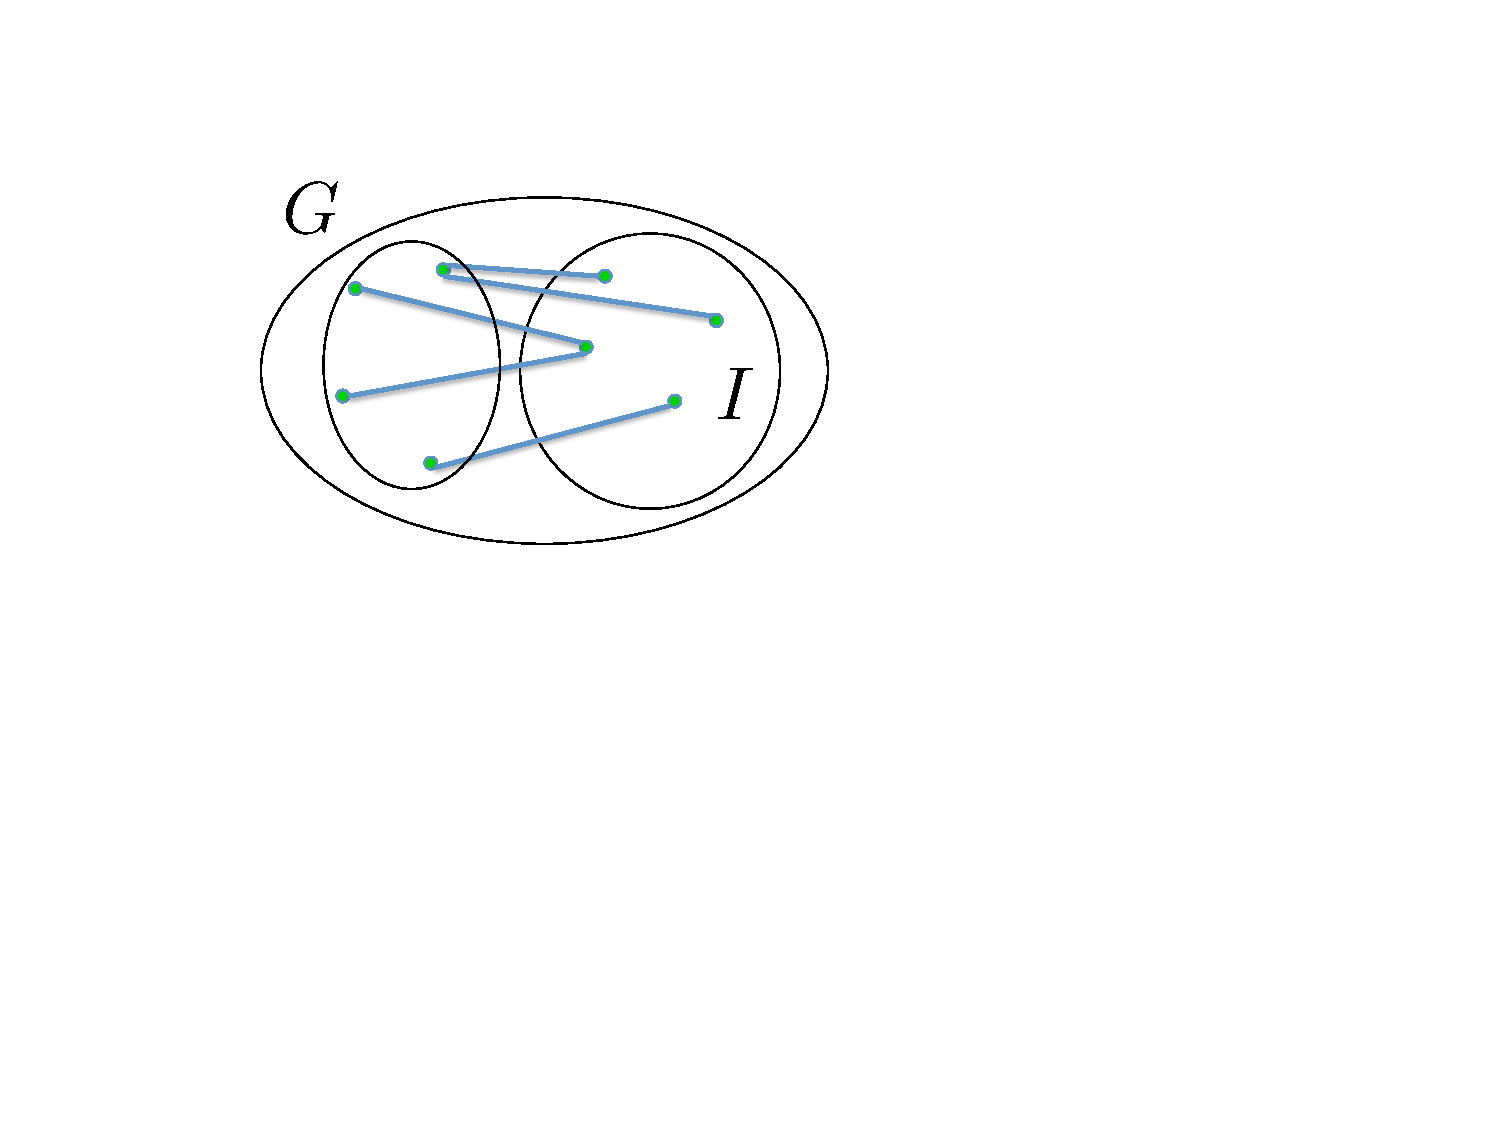
\includegraphics[scale=0.4]{idepmax02.pdf}
 \end{center}
 }

 $G=(V,E)$とするとき\\
 \[
  \begin{array}{l}
 \mathsf{adj}(G,v)=\{u|(u,v)\in E\}\\
 G\uparrow W=(V\cap W,E\cap(W\times W))
  \end{array}
 \]

\end{frame}

\begin{frame}
 \frametitle{彩色アルゴリズム:$Color(G,k)$}

 アイデア：独立集合$I$は一つの色=同じレジスタにわりあて
 
 $G\backslash I$:頂点集合$I$を削除し，$I$を端点に持つ辺を削除した
 グラフ

 \begin{center}
  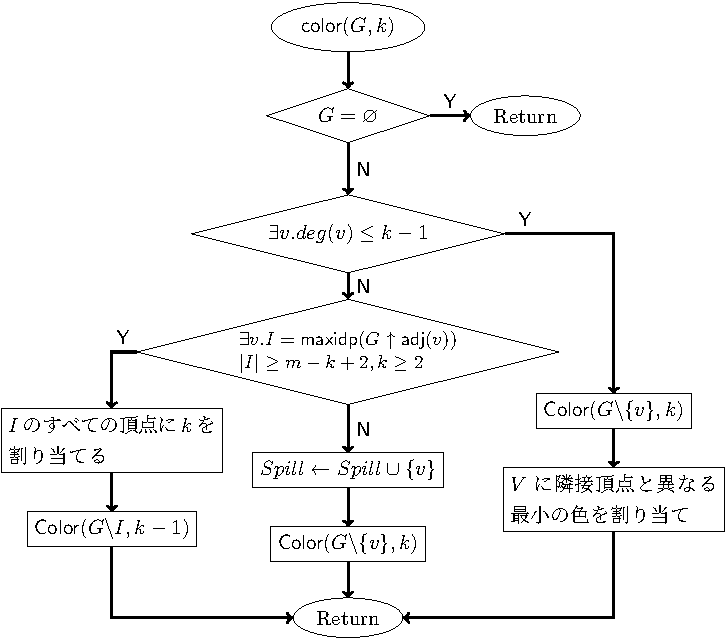
\includegraphics[height=.72\textheight]{algorithm7_7-crop.pdf}
 \end{center}
\end{frame}

\begin{frame}
 \frametitle{２部グラフ(bipartite graph)}
 
 \begin{Def}
  無向グラフ$G=(V,E)$が2部グラフであるとは，
  $V'\subseteq V$となる$V'$が存在して，$(u,v)\in E$に対して，
  $u\in V',v\in V\backslash V'$または$u\in V\backslash
  V',v\in V'$
 \end{Def}

 \begin{Prop}
  $G$が2彩色可能$\Leftrightarrow$$G$が2部グラフである
 \end{Prop}

 \begin{Lem}
  $G$が2部グラフである$\Leftrightarrow$$G$が奇数長の閉路を持たない
 \end{Lem}

 \greentext{木はbipartite graph=閉路がない}
 
 \begin{Thm}
  2彩色問題は線形時間で判定可能である．
 \end{Thm}

 \greentext{幅優先探索によって閉路探索を行う．このときに色を交互に変更
 する．}
 
\end{frame}
\begin{frame}
 \frametitle{隣接最大独立集合}

 $G':(U,E)=G\uparrow\mathsf{adj}(G,v)$の最大独立集合を求めるアルゴリズム

 \begin{center}
  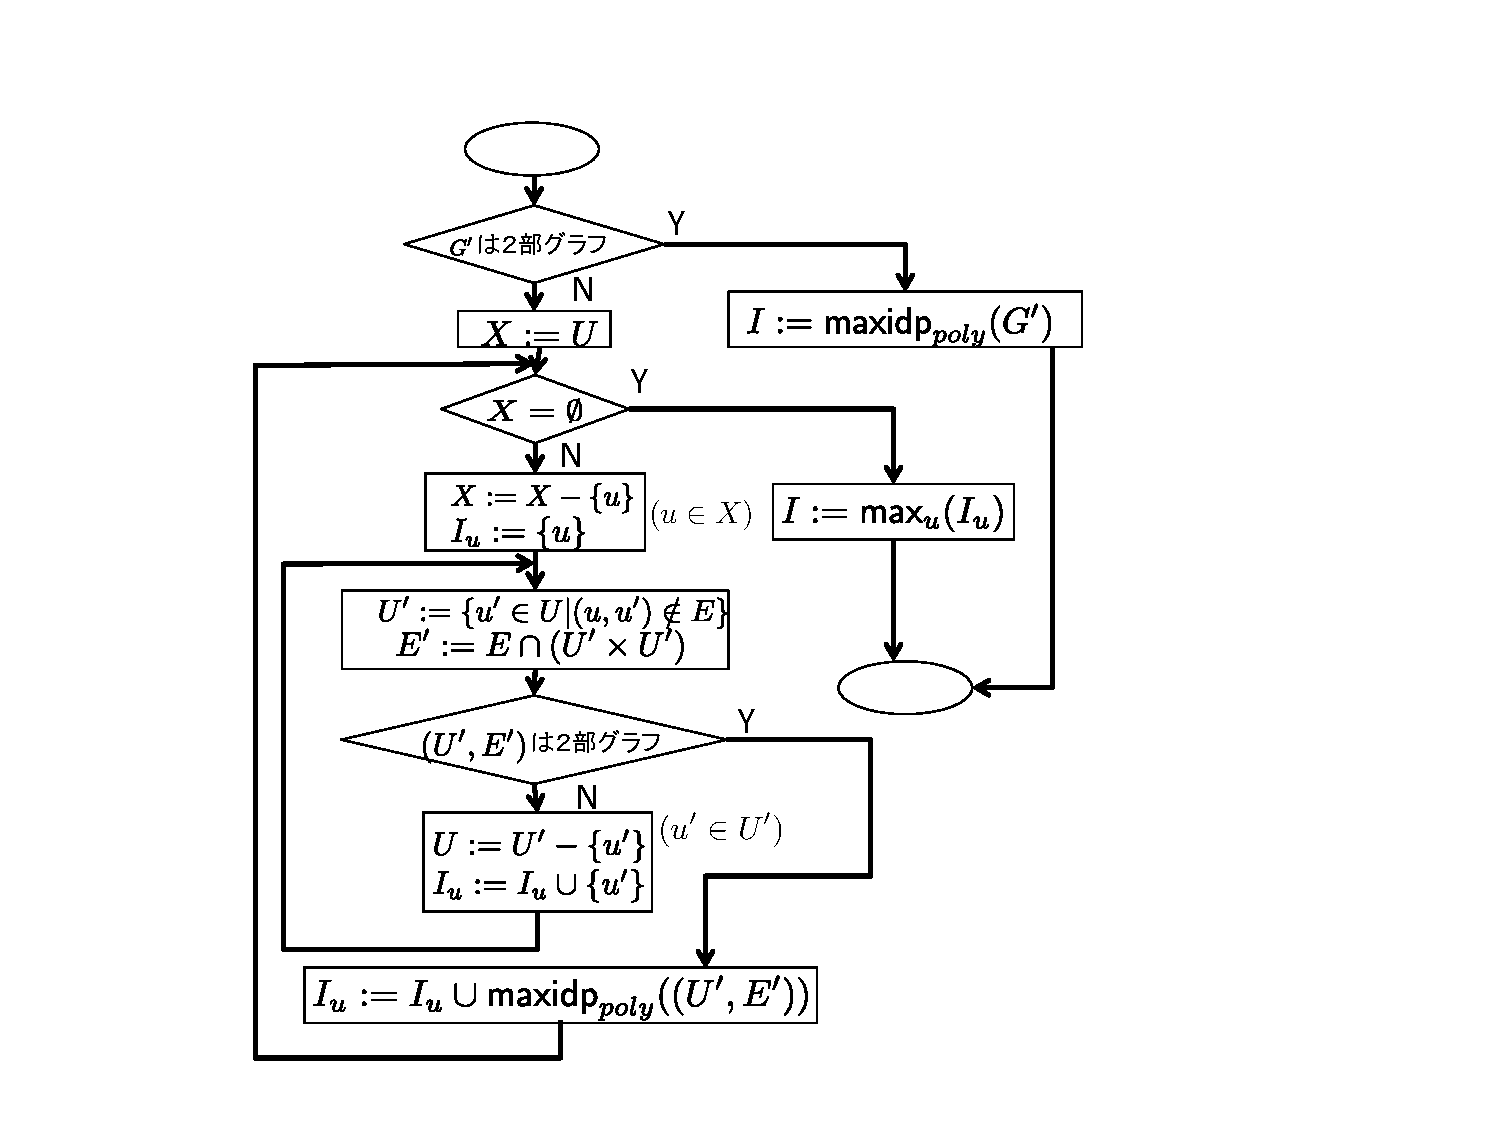
\includegraphics[height=.8\textheight]{alg7_8.pdf}
 \end{center}
 

\end{frame}

\begin{frame}
\frametitle{例}
\begin{center}
  \only<1>{
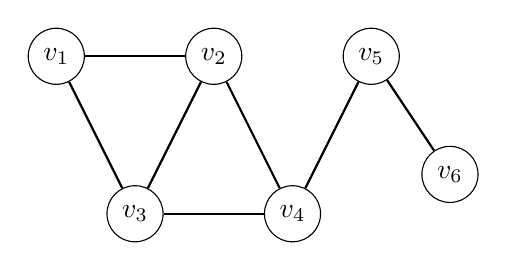
\begin{tikzpicture}[edge/.style={-, thick}]
    % 頂点の配置
    \node[draw,circle] (v1) at (0,2) {$v_1$};
    \node[draw,circle]  (v2) at (2,2) {$v_2$};
    \node[draw,circle]  (v3) at (1,0) {$v_3$};
    \node[draw,circle] (v4) at (3,0) {$v_4$};
    \node[draw,circle]  (v5) at (4,2) {$v_5$};
    \node[draw,circle] (v6) at (5,0.5) {$v_6$};

    % 辺の描画
    \draw[edge] (v1) -- (v2);
    \draw[edge] (v1) -- (v3);
    \draw[edge] (v2) -- (v3);
    \draw[edge] (v2) -- (v4);
    \draw[edge] (v3) -- (v4);
    \draw[edge] (v4) -- (v5);
    \draw[edge] (v5) -- (v6);
  \end{tikzpicture}

  \greentext{2部グラフではない}}
  \only<2>{
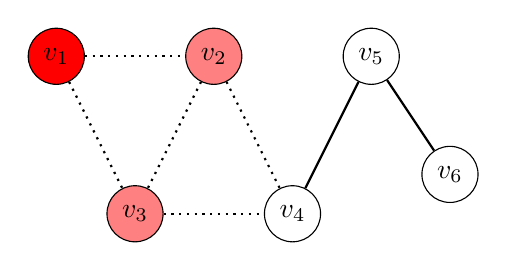
\begin{tikzpicture}[edge/.style={-, thick}]
    % 頂点の配置
    \node[draw,circle,fill=red] (v1) at (0,2) {$v_1$};
    \node[draw,circle,fill=red!50]  (v2) at (2,2) {$v_2$};
    \node[draw,circle,fill=red!50]  (v3) at (1,0) {$v_3$};
    \node[draw,circle] (v4) at (3,0) {$v_4$};
    \node[draw,circle]  (v5) at (4,2) {$v_5$};
    \node[draw,circle] (v6) at (5,0.5) {$v_6$};

    % 辺の描画
    \draw[edge,style=dotted] (v1) -- (v2);
    \draw[edge,style=dotted] (v1) -- (v3);
    \draw[edge,style=dotted] (v2) -- (v3);
    \draw[edge,style=dotted] (v2) -- (v4);
    \draw[edge,style=dotted] (v3) -- (v4);
    \draw[edge] (v4) -- (v5);
    \draw[edge] (v5) -- (v6);
  \end{tikzpicture}  
  
  \greentext{$v_1$を選んで直接到達できる頂点を消す．$I_{v_1}=\{v_1\}$}
  }
    \only<3,4>{
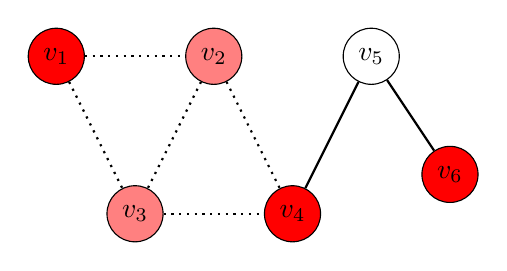
\begin{tikzpicture}[edge/.style={-, thick}]
    % 頂点の配置
    \node[draw,circle,fill=red] (v1) at (0,2) {$v_1$};
    \node[draw,circle,fill=red!50]  (v2) at (2,2) {$v_2$};
    \node[draw,circle,fill=red!50]  (v3) at (1,0) {$v_3$};
    \node[draw,circle,fill=red] (v4) at (3,0) {$v_4$};
    \node[draw,circle]  (v5) at (4,2) {$v_5$};
    \node[draw,circle,fill=red] (v6) at (5,0.5) {$v_6$};

    % 辺の描画
    \draw[edge,style=dotted] (v1) -- (v2);
    \draw[edge,style=dotted] (v1) -- (v3);
    \draw[edge,style=dotted] (v2) -- (v3);
    \draw[edge,style=dotted] (v2) -- (v4);
    \draw[edge,style=dotted] (v3) -- (v4);
    \draw[edge] (v4) -- (v5);
    \draw[edge] (v5) -- (v6);
  \end{tikzpicture}  
  
  \greentext{残りの頂点が2部グラフになった．最大独立頂点集合$\{v_4,v_6\}$\\$I_{v_1}=\{v_1,v_4,v_6\}$は独立頂点集合となる}
    }

    \uncover<4>{
  \redtext{この例では，$I_{v_1}$が最大独立頂点集合になる．}
  }
\end{center}
\end{frame}

\begin{frame}
 \frametitle{適用例}
 \only<1>{
 \begin{center}
  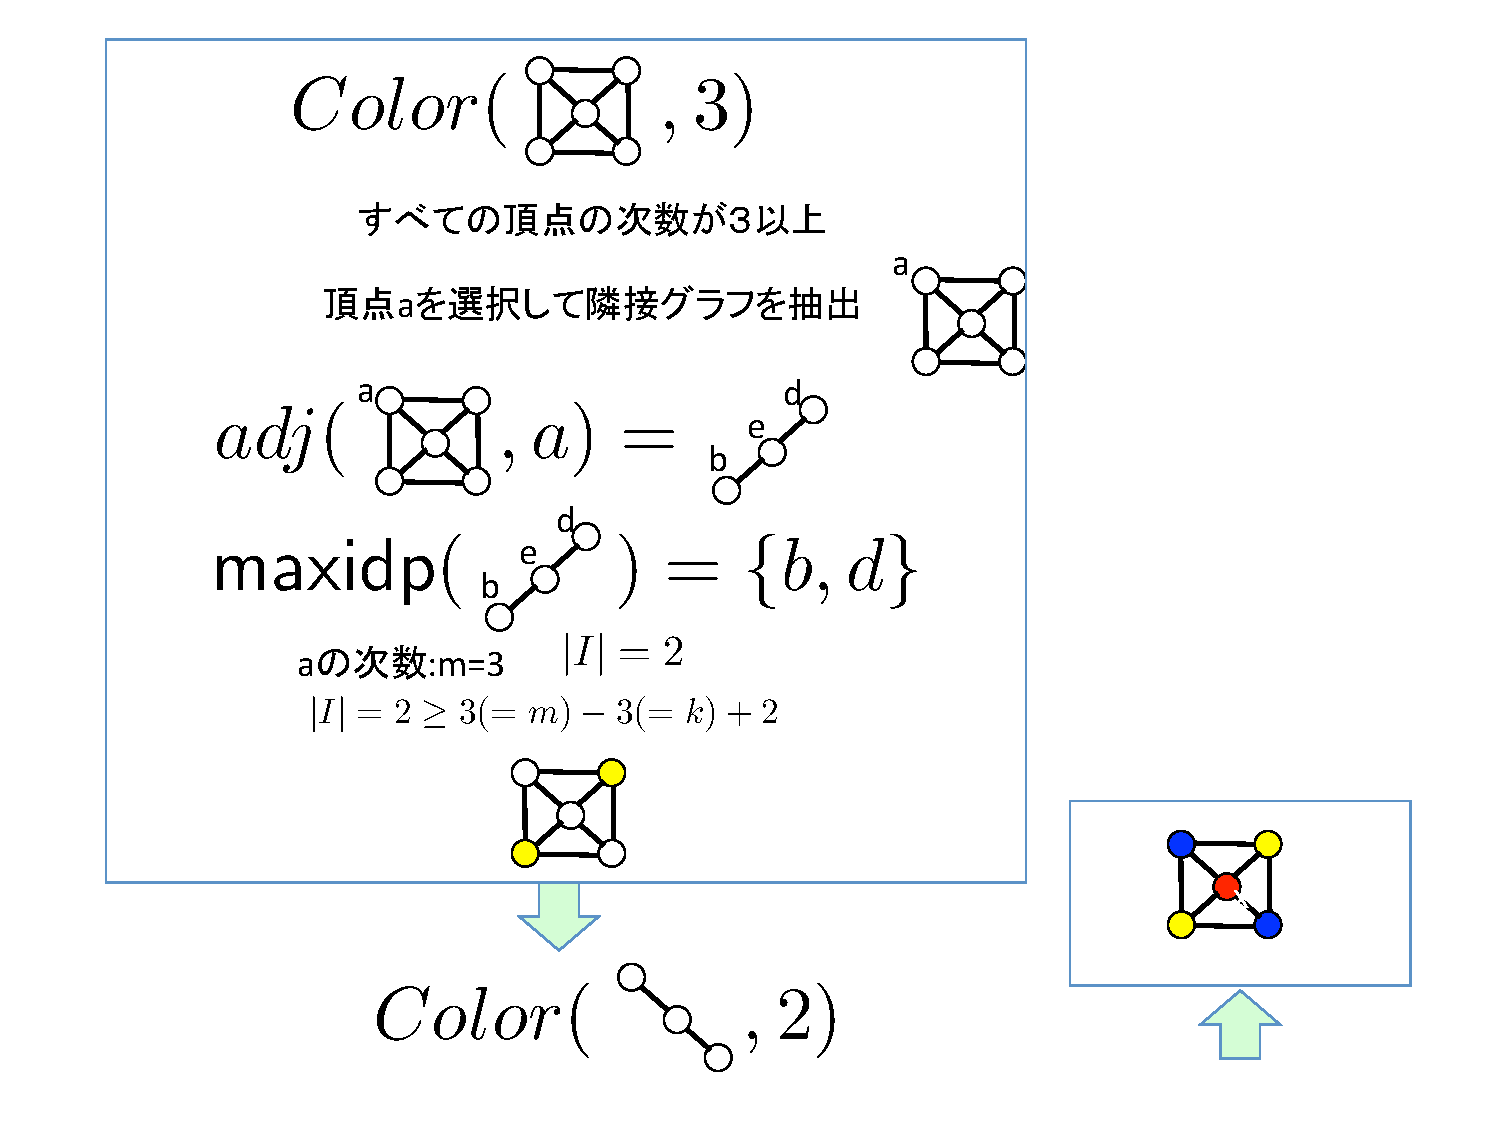
\includegraphics[height=.8\textheight]{gass01.pdf}
 \end{center}
 }
 \only<2>{
 \begin{center}
  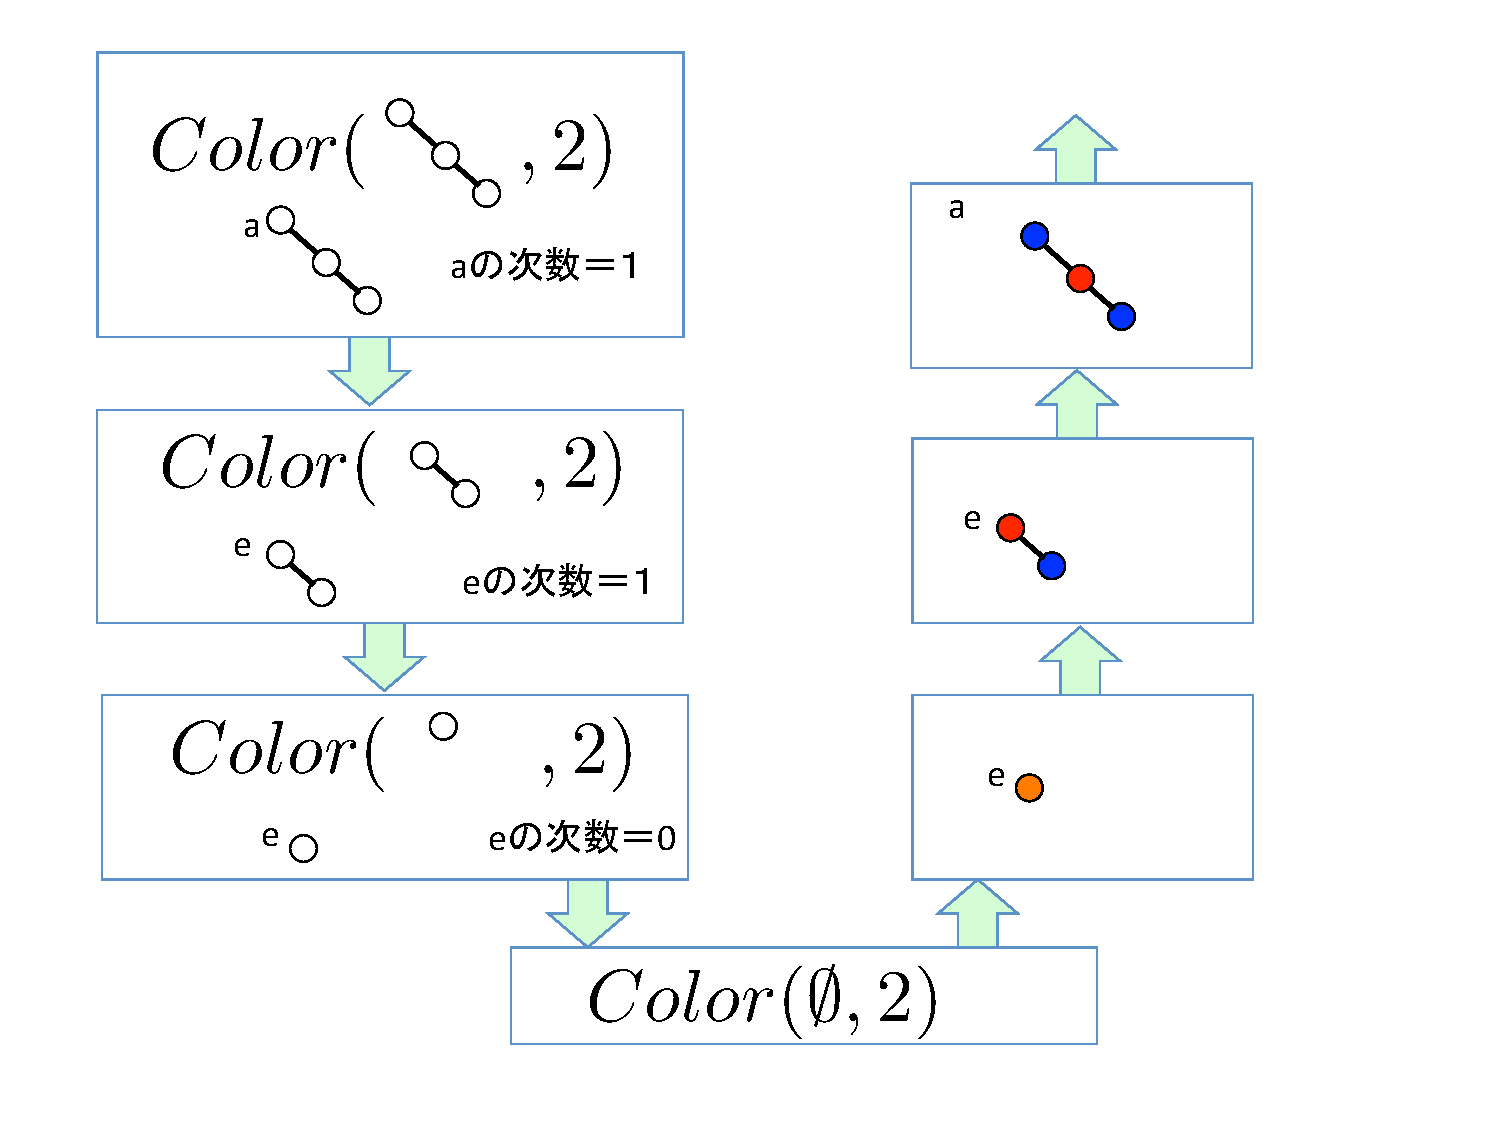
\includegraphics[height=.8\textheight]{gass02.pdf}
 \end{center}
 }
 
\end{frame}
\end{document}
